\begin{pa} \label{PA:10.4} 
  As we saw in Section \ref{S:9.5.Lines_Planes}, the equation
  of a plane passing through the point $(x_0, y_0, z_0)$ may be written
  as $A(x-x_0) + B(y-y_0) + C(z-z_0) = 0$.  If the
  plane is not vertical, then $C\neq 0$, and we can
  rearrange this as
  \begin{align*}
    C(z-z_0) & = -A(x-x_0) - B(y-y_0) \\
    z & = z_0-\frac AC(x-x_0) - \frac BC(y-y_0) \\
    z & = z_0 + a(x-x_0) + b(y-y_0)
  \end{align*}
  where we have written the constants $-A/C$ and $-B/C$ as $a$ and
  $b$, respectively.
  
  In this activity, we would like to understand the geometric
  significance of this expression.  We will consider the plane whose
  equation is the graph of the function $f(x,y)$:
  $$
  z = f(x,y) = 3 - \frac12(x-1) - 2(y-1).
  $$
  This plane is shown in Figure \ref{F:10.4.tangent.7}.  On the right,
  we have added the traces through the point $(x_0,y_0) = (1,1)$.
  
  \begin{figure}[ht]
    \begin{center}
      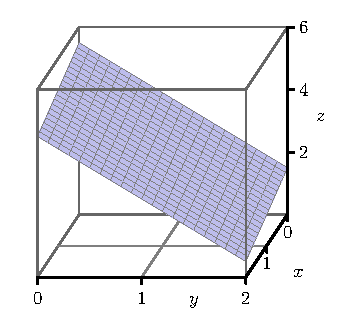
\includegraphics{figures/fig_10_4_tangent_8.eps}
      \hspace*{20pt}
      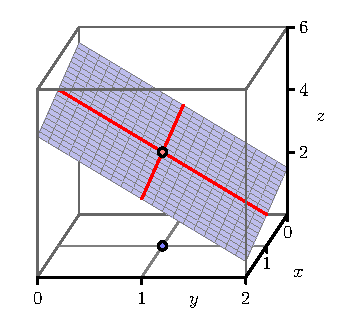
\includegraphics{figures/fig_10_4_tangent_7.eps}
    \end{center}
    \caption{The graph of $f(x,y)=3-\frac12(x-1)-2(y-1)$.}
    \label{F:10.4.tangent.7}
  \end{figure}

  \ba
  \item If $(x_0,y_0)=(1,1)$, what are the coordinates of the point on
    the plane above $(x_0,y_0)$?  How is this quantity reflected in
    the expression $z=z_0 + a(x-x_0) + b(y-y_0)$?

  \item Write the function $f(x, y_0) = f(x,1)$ that describes the
    trace of $f(x,y)$ with $y=y_0=1$.  Sketch its graph on the left of
    Figure \ref{F:10.4.preview.1}.  What is the slope of this trace?
    How is this slope related to the partial derivatives of $f$?  How
    does this slope appear in the expression $z=z_0 + a(x-x_0) +
    b(y-y_0)$? 

  \begin{figure}[ht]
    \begin{center}
      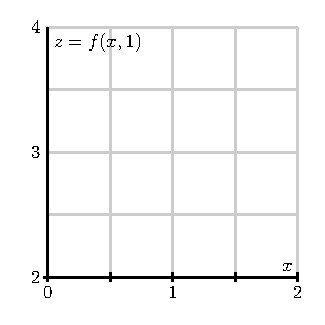
\includegraphics{figures/fig_10_4_preview_1.eps}
      \hspace*{20pt}
      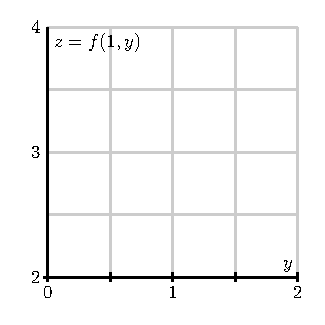
\includegraphics{figures/fig_10_4_preview_2.eps}
    \end{center}
    \caption{The traces of $f(x,y)=3-\frac12(x-1)-2(y-1)$.}
    \label{F:10.4.preview.1}
  \end{figure}

  \item Similarly, write the function $f(x_0, y) = f(1,y)$ that describes the
    trace of $f(x,y)$ with $x=x_0=1$.  Sketch its graph on the right of
    Figure \ref{F:10.4.preview.1}.  What is the slope of this trace?
    How is this slope related to the partial derivatives of $f$?  How
    does this slope appear in the expression $z=z_0 + a(x-x_0) +
    b(y-y_0)$? 

  \item If a plane is the graph of the function $z = f(x,y) = z_0 +
    a(x-x_0) + b(y-y_0)$, use the previous parts of this activity to
    explain why this may be written as 
    $$
    z = f(x_0, y_0) + f_x(x_0,y_0)(x-x_0) + f_y(x_0,y_0)(y-y_0).
    $$

  \ea



\end{pa} \afterpa 